\documentclass[10pt]{article}

\usepackage[utf8]{inputenc}
\usepackage[french]{babel}
%\usepackage[T1]{fontenc}
\usepackage{lmodern}
\usepackage{hyperref}
\usepackage{amsthm}
\usepackage{amscd}
\usepackage{mathtools}
\usepackage{amssymb}
\mathtoolsset{showonlyrefs=true}
\usepackage{fullpage}
\usepackage{graphicx}

%Il faut qu’on écrive une page ou deux par contre, pour expliquer le projet. En gros un titre,   
\title{Le modèle du COR amélioré}

\author{Bruno Scherrer}


\begin{document}

\maketitle

\section{Modèle du simulateur officiel du COR}

  Le modèle du COR repose sur un ensemble de $15$ variables numériques:
  \begin{itemize}
  \item $T$: niveau des cotisations sociales ;
  \item $P$: niveau des pensions par rapport aux salaires ;
  \item $A$: âge moyen de départ à la retraite ;
  \item $B$: part des revenus d'activités bruts dans le PIB ;
  \item $N_R$: Nombre de retraités de droit direct (tous régimes confondus) ;
  \item $N_C$: Nombre de personnes en emploi (ou nombre de cotisants) ;
  \item $G$: Effectif moyen d'une génération arrivant aux âges de la retraite ;
  \item $dP$: Autres dépenses de retraite rapportées au nombre de retraités de droit direct en \% du revenu d'activités brut moyen ;
  \item $T_R$: Taux des prélèvements sociaux sur les pensions de retraite ;
  \item $T_S$: Taux des prélèvements sociaux sur les salaires et revenus d'activité ;
  \item $C_{NV}$: Coefficient pour passer du ratio ``pensions/salaire moyen'' au ratio ``niveau de vie/salaire moyen'' ;
  \item $E_V$: Espérance de vie à 60 ans par génération ;
  \item $S$: Situation financière du système de retraite en \% du PIB ;
  \item $R_{NV}$: Niveau de vie des retraités par rapport à l'ensemble de la population ;
    \item $R_{EV}$: Durée de la vie passée à la retraite.
  \end{itemize}

~\\
  
  Sur le simulateur officiel du COR, toutes les variables ont, \emph{pour chaque scénario et l'ensemble des années}, des valeurs par défaut qui correspondent aux évolutions prévues dans le rapport du COR 2019 en l'absence de modification du système de retraite. Les 3 premières variables sont considérées comme des paramètres, à qui l'on peut donner de nouvelles valeurs $T'$, $P'$ et $A'$. Quand on modifie ces 3 degrés de liberté, la documentation du COR explique comment en déduire la modification induite sur les 3 dernières variables, qui prennent les valeurs $S'$, $R'_{NV}$ et $R'_{EV}$ (toutes les autres variables sont supposées fixes):

  \begin{align}
    S' &=  B [T-K(P'+dP)]\\
    R'_{NV} & = \frac{P' (1-T_R)C_{NV}}{1-(T_S+T'-T)}\\
    R'_{EV} & = \frac{ 60 + E -A' }{ 60 + E }
    \end{align}
  où on a noté:
  \begin{align}
    K & = \frac{N_R-G(A'-A)}{N_C+0,5G(A'-A)} \\
    E & = E_V \left\{~\mbox{arrondi}(\mbox{année}+1/2-A')~ \right\}
  \end{align}

  Les valeurs des \emph{variables fixes} selon le COR sont données à la Figure~\ref{conj}.
  \begin{figure}
    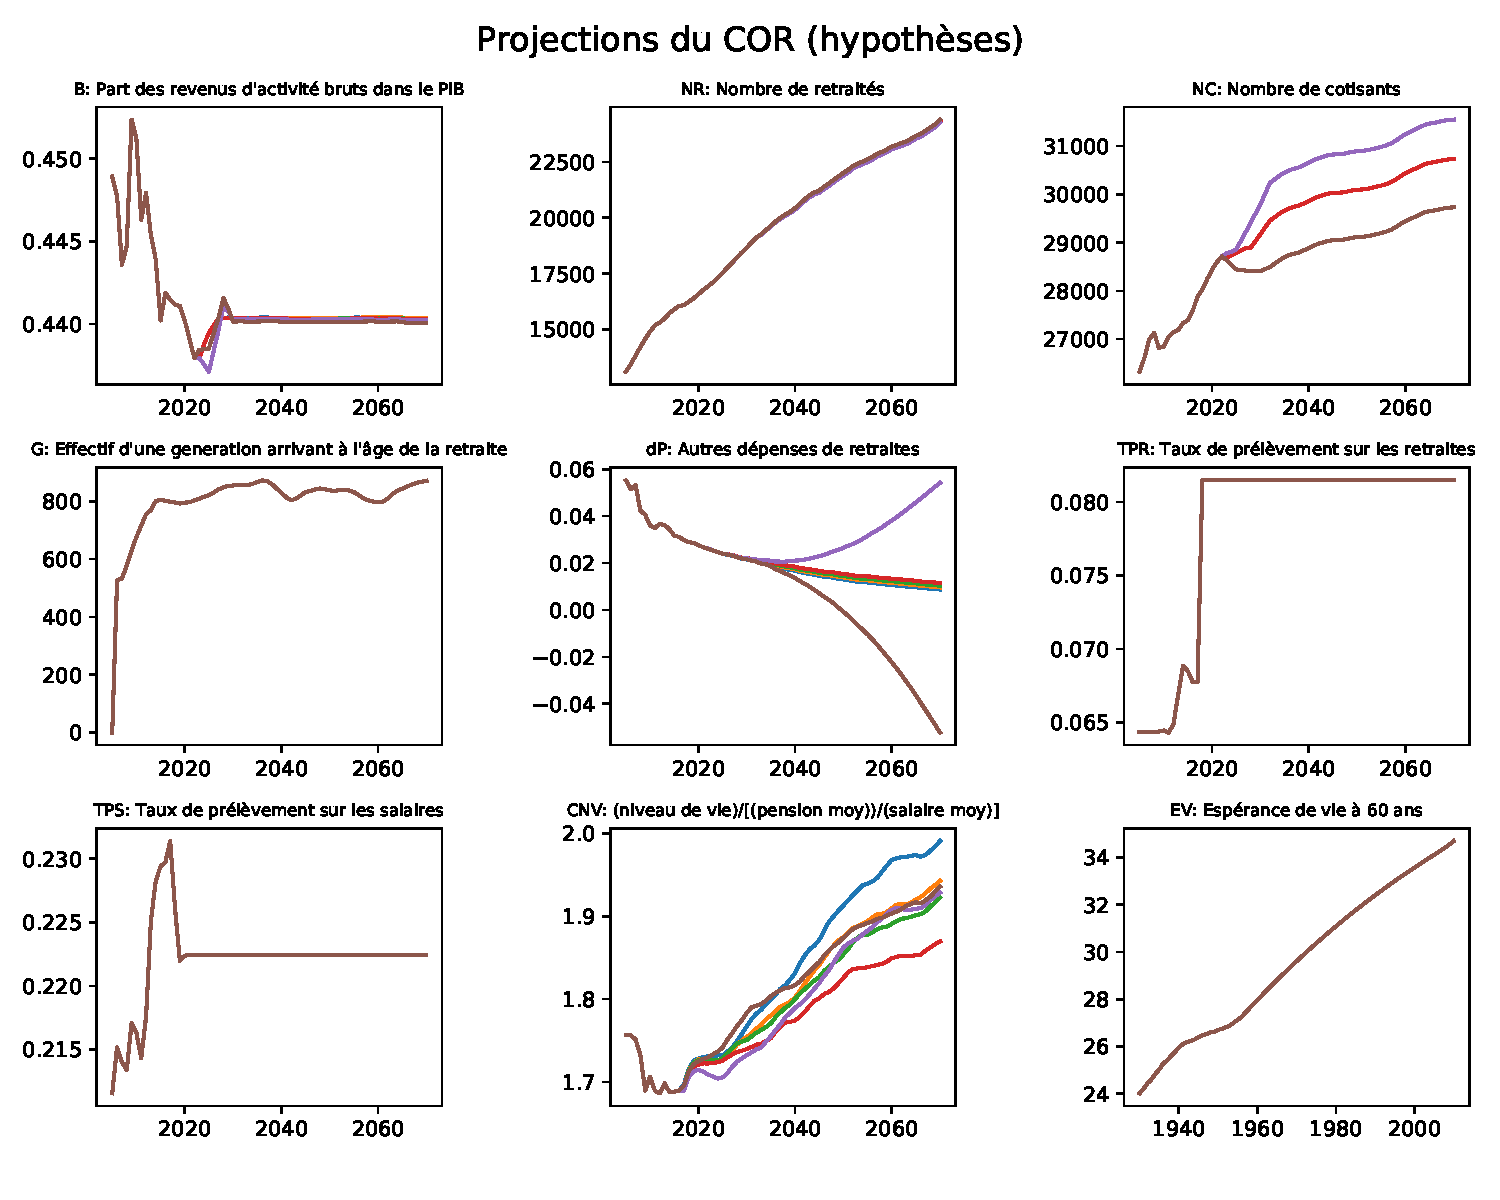
\includegraphics[width=20cm,angle=90]{conjoncture}
    \caption{\label{conj} Variables non contrôlables (COR)}
\end{figure}
  
  \section{Extensions}

  Dans ce qui suit, on donne les formules qui permettent de calculer $T'$, $P'$ et $A'$ lorsqu'on modifie d'autres paramètres.

  \subsection{Calcul de $T'$ et $P'$ à partir de $S'$, $R_{NV}'$ et $A'$}

  Ce calcul est utile lorsqu'on envisage une réforme à prestation définie, c'est-à-dire lorsqu'on choisit l'âge de départ à la retraite $A'$, une situation financière équilibrée $S'=0$, et un maintien du niveau de vie $R'_{NV}=1$.

  En inversant les formules plus haut, on obtient le niveau des pensions et le taux de cotisation nécessaires:
  \begin{align}
    P' &= \frac{U-S/B-KdP}{Z+K}, \\
    T' & = U-P'Z, \\
  \end{align}
  avec
  \begin{align}
    g & = G (A'-A), \\
    K & = \frac{N_R-g}{N_C + 0.5g}, \\
    Z & = \frac{ (1-T_R) C_{NV} }{R_{NV}}, \\
    U & = 1 - (T_S - T).
  \end{align}


\subsection{Calcul de $A'$ à partir de $P'$, $T'$ et $S'$}

  Ce calcul est utile lorsqu'on envisage une réforme où on contrôle les cotisations $T'$ (par exemple en gardant le niveau de dépenses prévues par le COR) et le niveau des pensions $P'$ (par exemple en considérant le maintien du niveau courant), tout en s'assurant que le système est équilibré financièrement ($S'=0$).

On déduit alors l'âge de départ à la retraite ainsi:
\begin{align}
     A' & = A + \frac{N_R - K N_C}{(0.5K+1)G}  \\
  \end{align}
  avec
  \begin{align}
    K = \frac{T'-S/B}{P'+dP}.
  \end{align}

  
  
  \subsection{Calcul de $P'$ à partir de $R'_{NV}$ et $T'$}

  Ce calcul est utile lorsqu'on veut contrôler les cotisations $T'$ et le niveau de vie $R'_{NV}$.

  Dans ce cas, on a:
  \begin{align}
    P' &= \frac{R'_{NV}[1-(T_S+T'-T)]}{C_{NV}(1-T_R)}. \\
  \end{align}


  \subsection{Calcul de $P'$ à partir de $T'$, $A'$ et $S'$}

  Ce calcul est utile lorsqu'on veut contrôler les cotisations $T'$ et l'âge de départ $A'$, tout en s'assurant que le système est équilibré financièrement ($S'=0$).

  On en déduit le niveau des pensions comme suit:
  \begin{align}
    P' = \frac{T-S/B}{K}-dP
  \end{align}
  avec
  \begin{align}
    g & = G (A'-A), \\
    K & = \frac{N_R-g}{N_C + 0.5g},
  \end{align}

  

  

\end{document}

